
\section{Dataset Introduction}
\label{sec:intro}

\subsection{Problem Description}

Credit card fraud detection problem is very important in large financial system. It is important that credit card companies are able to recognize fraudulent credit card transactions so that customers are not charged for items that they did not purchase.

The primary objective of this dataset is to enable the development and evaluation of effective credit card fraud detection models.Given the highly unbalanced nature of the dataset, with a small proportion of fraud cases, the challenge lies in accurately identifying instances of fraud while minimizing false positives. This imbalance poses a significant problem for machine learning algorithms to learn effectively.

Addressing this issue requires the development of advanced machine learning techniques, such as anomaly detection, class imbalance handling, or algorithmic adjustments for cost-sensitive learning. These approaches aim to improve the detection accuracy of fraudulent credit card transactions, ultimately benefiting both credit card companies and their customers by reducing financial losses and ensuring trust and security in financial transactions.

\subsection {Dataset Description}
The dataset in question contains credit card transactions made by European cardholders in September 2013. The purpose of this dataset is to aid credit card companies in recognizing fraudulent transactions to ensure that customers are not charged erroneously for purchases they did not make.

The dataset includes transactions that occurred over a period of two days, where there were 492 instances of fraud out of 284,807 total transactions. It is worth noting that the dataset is highly unbalanced, as the positive class (i.e. fraud) accounts for only 0.172\% of all transactions. This makes it particularly challenging to accurately predict instances of fraud.

The dataset consists solely of numerical variables resulting from a Principal Component Analysis (PCA) transformation. Aside from 'Time' and 'Amount', which were not transformed using PCA, features V1 through V28 represent the principal components obtained from the PCA analysis.

'Time' represents the elapsed time (in seconds) between each transaction and the first transaction in the dataset, while 'Amount' represents the amount of the transaction. The feature 'Class' is the response variable and takes a value of 1 if the transaction is identified as fraudulent, and 0 otherwise.

The visualization of the data yielded insightful results, indicating clear patterns and trends within the dataset. Through the use of graphical representations, we were able to identify key relationships between variables and draw meaningful conclusions from the data. These findings have practical implications, as they can inform decision-making in various fields, including business, healthcare, and policy-making.

\begin{figure}[h]
	\centering
	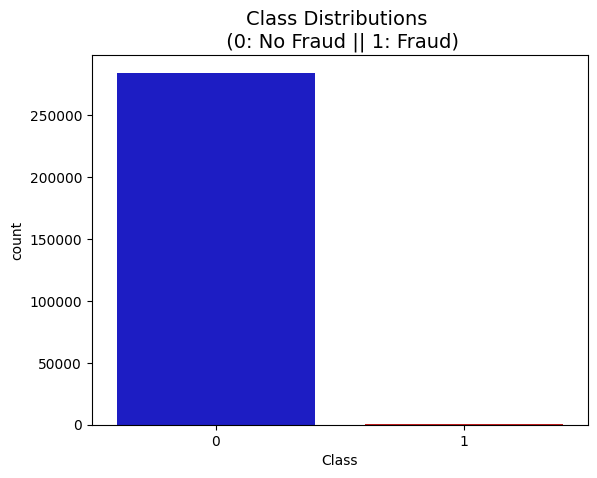
\includegraphics[width=0.7\linewidth]{../output7}
	\caption[Class Distribution]{Class Distribution}
	\label{Class Distribution}
\end{figure}

\begin{figure}[h]
	\centering
	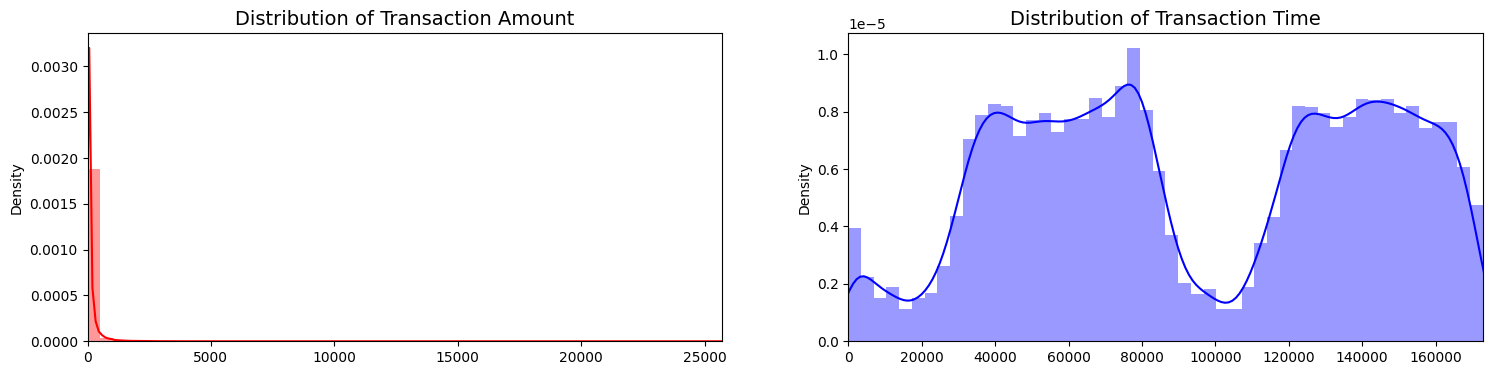
\includegraphics[width=0.7\linewidth]{../output8}
	\caption[Transaction Amount and Time Distribution ]{Transaction Amount and Time Distribution}
	\label{Transaction Amount and Time Distribution}
\end{figure}

\section{Outliers: Anomaly Detection}

\subsection{Introduction to Anomaly Detection}

Anomaly detection is a method of identifying observations or data that are considered unusual or abnormal compared to the rest of the dataset. The utilization of anomaly detection provides a crucial method for identifying unusual data points that provide insight into potential errors, fraud, or malicious activity. Anomalies often translate into significant business value, such as early identification of system failure, immediate responses against fraud, or preventing security breaches. The detection of anomalies requires various techniques and algorithms, including statistical methods, machine learning, and deep learning approaches. In general, identifying anomalies in data is a complex and challenging problem, as it often requires an understanding of the dataset and context of the application.

\subsection{Methods of Anomaly Detection}

The approaches for anomaly detection span a vast range of definitions and techniques, from rule-based methods to machine learning and deep learning algorithms. Traditionally, simple statistical techniques such as clustering, regression, or classification have commonly been employed to identify anomalies in data. More recently, unsupervised machine learning methods, including k-means, isolation forest, and one-class support vector machines, have gained popularity for detecting anomalies. Deep learning techniques, such as autoencoders, convolutional neural networks, and recurrent neural networks, can also detect anomalies by learning the data's underlying representations. Additionally, there are several open-source anomaly detection frameworks available, such as PyOD and Scikit-learn, which can aid in the implementation of these methods.

\subsubsection{Methods of Anomaly Detection:Interquartile Range Method}

\textbf{Introduction}

The Interquartile Range (IQR) method is a simple and robust method for detecting outliers in a dataset. The approach is based on the distribution's interquartile range, which is a measure of the dataset's spread. This method involves calculating the first (25th) and third (75th) quartiles of the dataset and then computing the distance between them. The distance, also referred to as the IQR, is then used to determine the threshold for classifying data points as outliers.

\textbf{Methodology}

The IQR method defines a data point as an outlier if it falls outside the range of the \textit{inner fence}, which is defined as:

\begin{equation} \textrm{Inner fence} = [\textrm{Q1} - k(\textrm{IQR}), \textrm{Q3} + k(\textrm{IQR})] \end{equation}

where Q1 and Q3 are the first and third quartiles of the dataset, respectively, and k is a scaling factor that determines the range of the inner fence. Typically, k is set to 1.5, but it can be adjusted based on the specific dataset and problem.

Data points outside the inner fence but within the \textit{outer fence} are considered mild outliers, while those above the outer fence are classified as extreme outliers. The outer fence is defined as:

\begin{equation} \textrm{Outer fence} = [\textrm{Q1} - 3k(\textrm{IQR}), \textrm{Q3} + 3k(\textrm{IQR})] \end{equation}

The IQR method is simple to implement and computationally efficient, making it a popular choice for detecting outliers. However, it requires that the data be roughly symmetrically distributed, and it is less effective at detecting outliers in skewed distributions.


\textbf{Experiment Results :}

We have to be careful as to how far do we want the threshold for removing outliers. We determine the threshold by multiplying a number (ex: 1.5) by the (Interquartile Range). The higher this threshold is, the less outliers will detect (multiplying by a higher number ex: 3), and the lower this threshold is the more outliers it will detect.  

\begin{figure}[h]
	\centering
	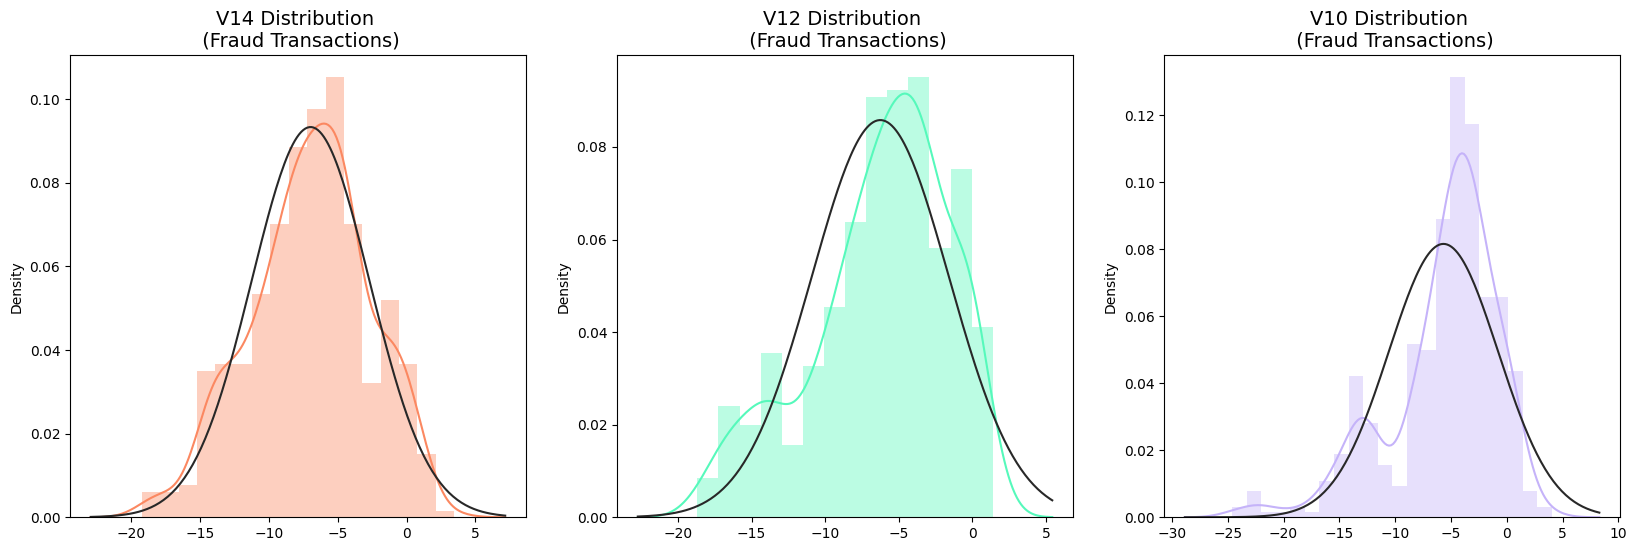
\includegraphics[width=0.7\linewidth]{../output9}
	\caption{}
	\label{Visualization of feature distribution}
\end{figure}


**The Tradeoff: **

The lower the threshold the more outliers it will remove however, we want to focus more on "extreme outliers" rather than just outliers. We might run the risk of information loss which will cause our models to have a lower accuracy. 

 We first start by visualizing the distribution of the feature we are going to use to eliminate some of the outliers. V14 is the only feature that has a Gaussian distribution compared to features V12 and V10.
 
 After we decide which number we will use to multiply with the iqr (the lower more outliers removed), we will proceed in determining the upper and lower thresholds by substrating q25 - threshold (lower extreme threshold) and adding q75 + threshold (upper extreme threshold).

\begin{figure}[h]
	\centering
	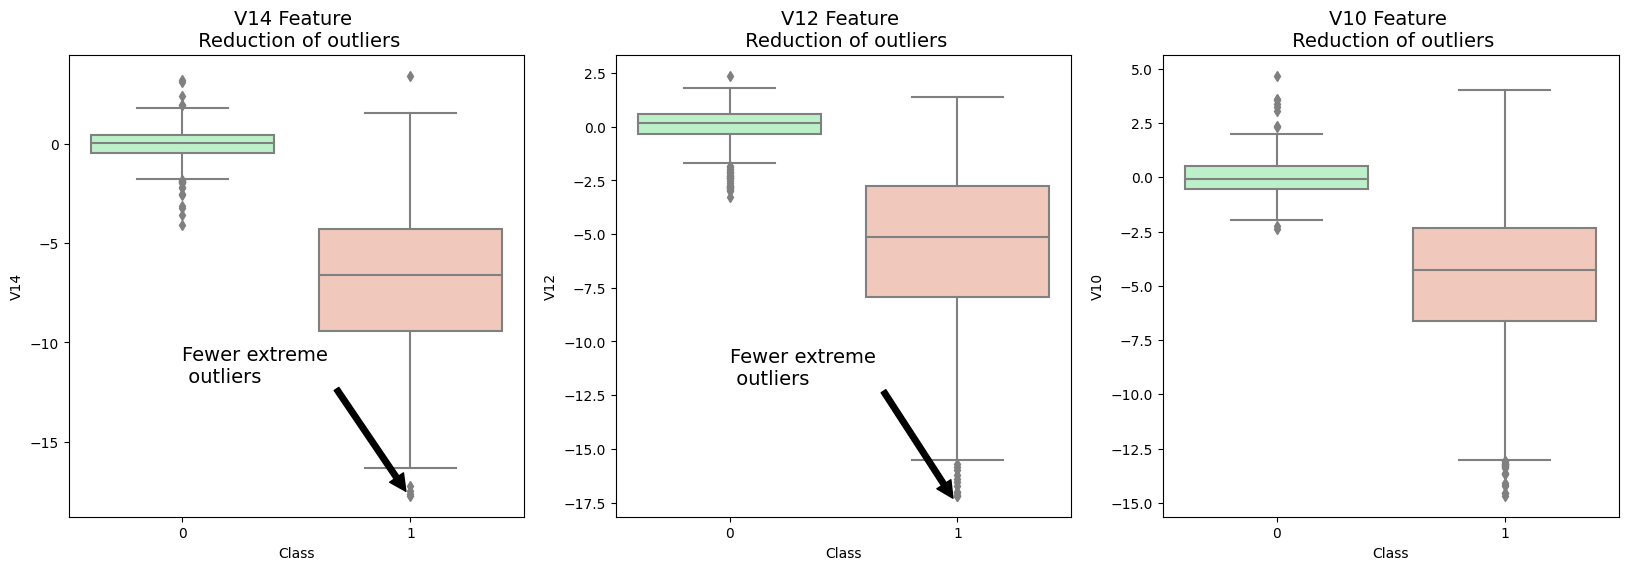
\includegraphics[width=0.7\linewidth]{../output10}
	\caption{}
	\label{Visualization of Outliers}
\end{figure}


\section{Class Imblance Handling Approach}


\section{Machine Learning Theory}

To solve this problem, we need to build a model that can detect fraudulent transactions based on the features. One possible method is to use a logistic regression model, which is a type of supervised learning algorithm that can perform binary classification. The logistic regression model estimates the probability of a transaction being fraudulent using a sigmoid function:

\subsection{Logistic Regression}



\[p(y=1|x) = \frac{1}{1+e^{-\theta^Tx}}\]

where $x$ is the feature vector, $\theta$ is the parameter vector and $y$ is the class label.

To train the logistic regression model, we need to find the optimal values of $\theta$ that minimize the cost function, which is defined as:

\[J(\theta) = -\frac{1}{m}\sum_{i=1}^m[y^{(i)}\log(p(y^{(i)}=1|x^{(i)}))+(1-y^{(i)})\log(1-p(y^{(i)}=1|x^{(i)}))]\]

where $m$ is the number of training examples.

We can use an optimization algorithm such as gradient descent to update $\theta$ iteratively until convergence:

\[\theta := \theta - \alpha \frac{\partial J(\theta)}{\partial \theta}\]

where $\alpha$ is the learning rate.

However, since the dataset is highly unbalanced, we may need to apply some techniques to deal with the class imbalance problem, such as oversampling, undersampling or using a weighted cost function. These techniques can help improve the performance of the model and reduce the bias towards the majority class.






\section{Summary}



% R code here if necessary \begin{lstlisting}[style=cmd]
	% load('mydata.Rdata')
	% \end{lstlisting}
% \ \\

% Output of the code
% \begin{lstlisting}[style=output]
	%  this is a code in output style ...
	% \end{lstlisting}
% \ \\
% Code inline
% \lstinline[style=cmd]|this is an inline code ...|\\
% \ \\

% To add an image:
% 
\includegraphics[scale=0.5]{logoDMI.jpg} % save images in the folder img


